\subsection{Introduction to Complex Numbers}
In mathematics, a complex number is an element of a number system that extends the real numbers
with a specific element denoted i, called the imaginary unit and satisfying the equation i²= -1; every
complex number can be expressed in the form a + bi, where a and b are real numbers.

% draw a table of complex numbers i powers
\begin{center}
\begin{tabular}{|c|c|}    
    \hline	
    $i$ & $\sqrt{-1}$ \\ \hline
    $i^2$ & $-1$ \\ \hline
    $i^3$ & $-i$ \\ \hline
    $i^4$ & $1$ \\ \hline
    $i^5$ & $i$ \\ \hline
    $i^6$ & $-i$ \\ \hline
    $i^7$ & $-1$ \\ \hline
    $i^8$ & $i$ \\ \hline
\end{tabular}
\end{center}

% describe table
\begin{center}
    $i$ Chart.
\end{center}

If you look at the table, you can see that the imaginary unit is the $\sqrt{-1}$. Going down the chart you can see there is a pattern till the $i^n$ where $n$ is the power of the imaginary unit.

Remember at least the first 4 powers of the imaginary unit. Later we will use it to evaluate the complex numbers into the form $a+bi$.

\subsection{Graphing Complex Numbers}
In mathematics, the complex plane is the plane formed by the complex numbers, with a Cartesian coordinate system such that the x-axis, called real axis, is formed by the real numbers, and the y-axis, called imaginary axis, is formed by the imaginary numbers. 


% show image
\begin{figure}[h!]
    \centering
    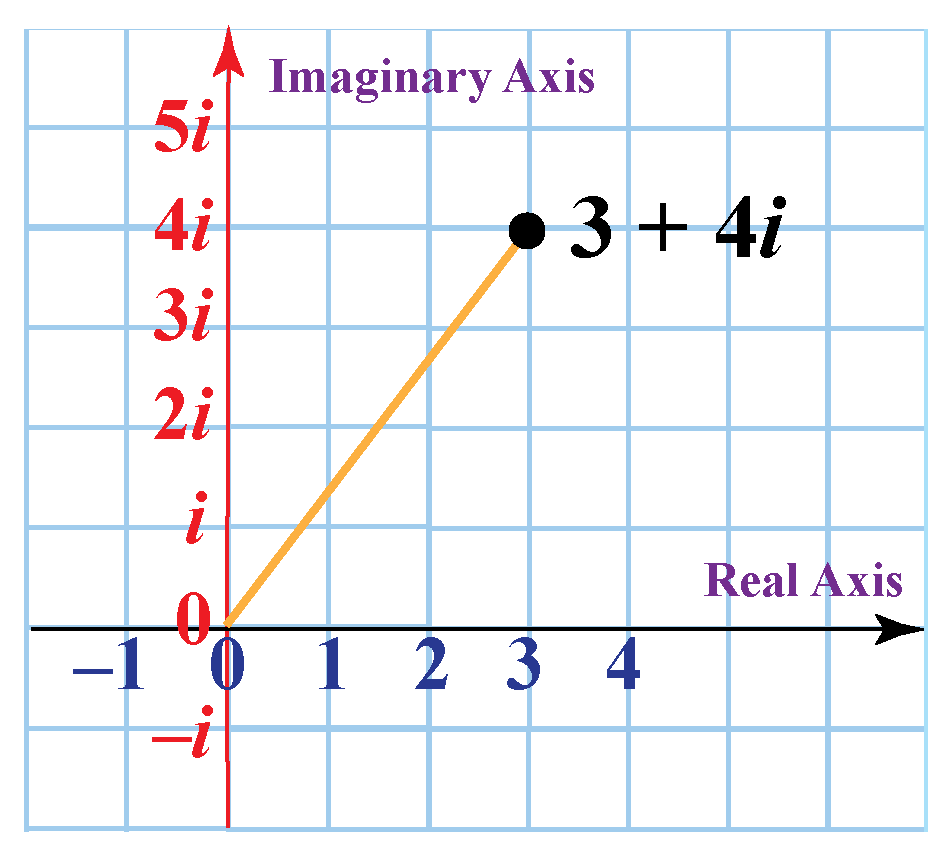
\includegraphics[width=0.35\textwidth]{graphingcomplexnumbers.png}
    \caption{Complex plane}    
\end{figure}

I will come back to this later. We will use this tool in converting standard complex numbers into the polar form $r$ and $\theta$.


\subsection{Operations with Complex Numbers}

\subsubsection{Addition}

To add two complex numbers, add the real part to the real part and the imaginary part to the imaginary part.

\begin{equation}
    (a+bi)+(c+di)=(a+c)+(b+d)i
\end{equation}

Example: $(2+7i)+(3-4i)$

\begin{equation}
    (2+7i)+(3-4i)=(2+3)+(7+(-4))i
    =5+3i
\end{equation}

\subsubsection{Subtraction}
To substract two complex numbers, substract the real part to the real part and the imaginary part to the imaginary part.

\begin{equation}
    (a+bi)-(c+di)=(a-c)+(b-d)i     
\end{equation}

Example: $(2+7i)-(3-4i)$

\begin{equation}
    (2+7i)-(3-4i)=(2-3)+(7+4i)i
    =5+(-3)i
\end{equation}

\subsubsection{Multiplication}
Multiplication of two complex numbers is defined as:
\begin{equation}
    (a+bi)(c+di)=(ac-bd)+(ad+bc)i
\end{equation}

Example: $(2+7i)(3-4i)$

\begin{equation}
    \begin{split}        
(2+7i)(3-4i)=(2*3-4*7)+(2*4+7*3)i\\
=(-10+28)+(12+(-7))i \\
=18+(-7)i            
    \end{split}
\end{equation}

\subsubsection{Conjugate}
Conjugate of a complex number is defined as:
\let\conjugatet\overline
\begin{equation}
    \begin{split}
        \conjugatet{(a+bi)}=a-bi\\
    \end{split}
\end{equation}

Example: $\conjugatet{(2+7i)}$

\begin{equation}
    \begin{split}
        \conjugatet{(2+7i)}=2-7i
    \end{split}
\end{equation}

\begin{center}
    Notice that only the sign between the real and imaginary part is changed oppositely.
\end{center}

\subsubsection{Division}
Division of two complex numbers is defined as:
\begin{equation}
    \begin{split}
    \frac{(a+bi)}{(c+di)} = \frac{(a+bi)(c-di)} {(c+di)(c-di)}\\
    = \frac{(a+bi)(c-di)} {(c^2+d^2)}\\
    = \frac{(a+bi)}{(c^2+d^2)} + \frac{(c-di)}{(c^2+d^2)}i\\    
    \end{split}
\end{equation}

Example: $\frac{(2+7i)}{(3-4i)}$

\begin{equation}
    \begin{split}
    \frac{(2+7i)(3+4i)}{(3-4i)(3+4i)} = \frac{-22+29i}{25}
    = -\frac{22}{25} + \frac{29}{25}i
    \end{split}
\end{equation}



\subsubsection{Modulus}
Finding the modulus of a complex number. \\\\
General formula for Modulus of $a+bi$ is:
\begin{equation}
    \sqrt{a^2+b^2}
\end{equation}

Example : Find the modulus of -4 + 3i.

\begin{equation}
    Modulus = \sqrt{(-4)^2+(3)^2}=\sqrt{25}=5
\end{equation}

\subsection{Computing $i^n$ Complex Numbers}

Remember the first 4 powers of the imaginary unit now we are going to use it to evaluate the complex numbers.

Example: Evaluate $i^{105}$

\begin{equation}
    \begin{split}
        i^{105} = i^{104}*i \\
        i^{104} = (i^2)^{54} \\
        i^{104} = (-1)^{54} = 1\\
        \therefore i^{105} = i
    \end{split}
\end{equation}

Example: Evaluate $i^{647}$
\begin{equation}
    \begin{split}
        i^{647} = i^{646}*i \\
        i^{646} = (i^2)^{323} \\
        i^{646} = (-1)^{323} = -1\\
        \therefore i^{647} = -i
    \end{split}
\end{equation}

Example: Evaluate $i^{142}$
\begin{equation}
    \begin{split}
        i^{142} = (i^2)^{71} \\
        i^{142} = (-1)^{71} = -1\\        
        \therefore i^{142} = -1
    \end{split}
\end{equation}

Bonus: Evaulating $(-1)^n$.

\begin{equation}
    (-1)^n =
    \left\{
        \begin{array}{lr}
            1, & \text{if } n \in \{n=2n | n \in \mathbb{N} \} \\
            -1, & \text{if } n \in \{n=2n+1 | n \in \mathbb{N} \}
        \end{array}
    \right\} 
\end{equation}

\subsection{Complex Numbers in the Polar Form}

The polar form of a complex number $z = x + iy$ with coordinates $(x, y)$ is given as $z = r\cos{\theta} + ir\sin{\theta} = r(\cos{\theta}+i\sin{\theta})$. The abbreviated polar form of a complex number is $z = rcis(\theta)$, where $r = \sqrt{x^{2}+y^{2}}$ and $\theta = \arctan{(\frac{r}{x})}$. \\

Example: Express the complex number in polar form.

$5+2i$

\begin{equation}
    \begin{split}
        r = \sqrt{5^2+2^2} = \sqrt{29} = 5.39 \\
        \text{now find $\theta$} \\ 
        \angle = \arctan{(\frac{2}{5})}  = 21.80^{\circ} \\ 
        \text{to find the correct $\theta$ we have to use the Argand diagram to see which quadrant the $\theta$ lies in.} \\
        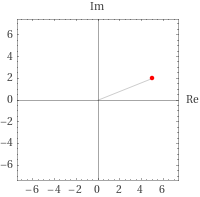
\includegraphics[width=0.25\textwidth]{argand.png} \\
        \text{The quadrant is $1$ the $\theta$ will remain the same as the ref $\angle$} \\
        \text{$\theta$ is $21.80^{\circ}$} \\
        \text{later below this section i will propose all the cases to work out $\theta$ due to different quadrant numbers} \\
        \text{The polar form of the complex number is:} \\
        5.39(\cos{(21.80)^{\circ}}+i\sin{(21.80)^{\circ}}) \\        
        \text{where $\theta$ is measured in degrees.} \\
    \end{split}
\end{equation}

\subsubsection{Working out $\theta$ in different quadrants}

Lets denote the quadrant number as $q_{n}$ and the ref angle as $\angle$.

\begin{equation}
    \theta =
    \left\{
        \begin{array}{lr}
            \angle, & \text{if } q_{1}\\
            180-\angle^{\circ}, & \text{if } q_{2} \\
            180+\angle^{\circ}, & \text{if } q_{3} \\
            360-\angle^{\circ}, & \text{if } q_{4} \\                        
        \end{array}
    \right\} 
\end{equation}